\documentclass[conference]{IEEEtran}

\usepackage{graphicx}
\graphicspath{ {./images/} }
\usepackage{caption}
\usepackage{subcaption}
\captionsetup[subfigure]{justification=centering}

\begin{document}

\title{Automated Conversion of Sketches into Source Game Engine Maps}
\author{
\IEEEauthorblockN{Cameron Stevenson}
\IEEEauthorblockA{Dept. Computer Science and Software Engineering\\
University of Canterbury\\
Christchurch, New Zealand\\
Email: cst122@uclive.ac.nz}
\and
\IEEEauthorblockN{Richard Green}
\IEEEauthorblockA{Dept. Computer Science and Software Engineering\\
University of Canterbury\\
Christchurch, New Zealand\\
Email: richard.green@canterbury.ac.nz}
}

 \maketitle
 
\begin{abstract}
This paper proposes a method to automatically generate Source game engine maps from hand sketched layouts. Segmentation of regions inside pencil is achieved through adaptive thresholding and flood fill, with an 8\% difference from a reference segmentation. Text recognition is achieved through squared difference template matching of individual letters, with 100\% detection and recognition and no false detections. A compilable and playable CS:GO map is generated.
\end{abstract}

\section{Introduction}

Video games made by Valve run on the Source game engine, and share a common map editor and map file specification. Counter Strike: Global Offensive (CS:GO) is one such game, which has many past and present community-made maps for the competitive game mode. The map editor operates in 3D and is more suited to blocking in finer details. Blocking in the basic layout of the map can be time consuming, especially with complex geometry such as curves. If the process of taking a 2D layout idea and making a 3D map from it were automated, it would free up creative potential for map authors. This paper aims to automatically interpret sketched layouts to create the geometry and entities necessary to have a compilable and playable map.

\section{Background}
\subsection{Text Detection and Recognition}
Rosebrock \cite{rosebrock2018opencv} and others detail a method of detecting text bounding boxes with EAST, and recognising words with Tesseract. EAST is capable of detecting word and line text in natural backgrounds \cite{zhou2017east}. Tesseract \cite{smith2007overview} is Google's text recognition engine which maintains uncertainty throughout the letter recognition process until words are recognised. Feeding the bounding boxes found by EAST into Tesseract is usually a robust method of recognising font text in real images. However the training is based on words and computer fonts, so it may fail on handwritten letters.

Methods exist for recognising handwritten characters from different people. Pal et al. \cite{pal2010handwritten} skeletonize characters and use neural networks to recognise characters. This method operates on images of single characters, limiting it to situations where bounding boxes have already been established.

General shape similarity methods may be applied, such as those found in Skiena's book \cite{skiena2020algorithm}. Hamming distance of two shapes is how much they don't overlap in area when placed on top of each other. This fails to account for scale, shift, skew, and rotation. Hausdorff distance focusses on the place where 2 shapes differ the most, measuring the furthest distance you can be from one shape if you lie on the furthest point in the other shape. Skeleton comparison reduces shapes to their core structure, then compares topology and length/angle features.

\subsection{Sketch Interpretation}

Naya et al. \cite{naya2002direct} recognise the need for allowing users to sketch designs before converting them into computer models. Their proposal shows how sketched lines can be interpreted within certain tolerances to give digital representations. However it only works for straight lines.

Similarly Zargar et al. \cite{zargar2019introducing} interpret perspective sketches to generate 3D models. Again it only works for straight lines.

Yetiş et al. \cite{yetics2019auto} observe that freeform sketches generally rely on human experience to resolve ambiguities when interpreting their meaning. Also, discontinuities and irregularity in lines can cause imprecise models. They attempt to use deep learning in the 2D to 3D conversion, and it gets the basic outline of architectural sketches correct. It is limited to the features it has been trained on.

\subsection{Polygon Simplifcation}

Polygons sourced from real life data (such as a photo scan) can have more points representing them than practically necessary. Polygon simplification adds, removes or modifies vertices to produce a similar enough polygon with much fewer vertices.

The Douglas-Peucker algorithm \cite{douglas1973algorithms} for polygon simplification is additive. It begins with 2 points of the original polygon, and adds other points from the original polygon which are sufficiently far from the current approximation. Once every non-added point is sufficiently close to the approximation, it terminates. The worst case scenario is inefficient when an approximation polygon has almost the same number of vertices as the original (when the original polygon is complicated).

Other techniques subtract points from low area or large angle triangles along the polygon.

\subsection{Polygon Triangulation}

Many applications use triangles as primitives, so breaking down a polygon into triangles is useful.

A typical triangulation has $n-2$ triangles for $n$ vertices. Asano et al. \cite{asano1986polygon} demonstrate how collinearity of vertices can be used to minimise triangle count beyond $n-2$, at the cost of time complexity. Triangulation cannot be faster than sorting. 

Shewchuk's Triangle \cite{shewchuk2005two} creates Delaunay triangulations, optionally with no large or small angles. Delaunay triangulations spread out triangles fairly evenly throughout the polygon.

\subsection{Valve Maps}

Valve Map Format \cite{valve2006vmf} describes the structure of an editable map file. It has a key-value structure with nesting, similar to JSON. Of particular interest is the brush, referred to as "solid" in this wiki. A brush is a convex 3D shape, defined by a number of sides making up its shape within them. Each side is a plane, and where these planes intersect create the vertices and edges of the brush.

CS:GO maps tend to have 1 buyzone for each team (and player spawns), 1-3 bombsites, floors connecting main areas, walls dividing main areas, and a skybox surrounding the map. I have coloured the segmented sketch as follows (see Figure \ref{fig:segtest} for an example).
\begin{itemize}
\item Green: Floor
\item Red: Wall
\item Yellow: Bombsites
\item Blue: CT Spawn
\item Orange: T Spawn
\end{itemize}

\section{Proposed Method}
\subsection{Segmentation}
We aim to find the segments divided by pencil lines.

The sketch is grayed, inverted, and blurred. An adaptive threshold highlights both sides of each pencil mark as black, with the background in white. This is inverted so pencil edges are white against a black background. A closing operation with 2 dilations and 1 erosion of a 5x5 kernel joins the two sides of each pencil mark, giving thick white pencil against a black background. These white edges may contain black pixels within them. This is acceptable as long as the edge has no black path between segments. See Figure \ref{fig:seg}.

Now that black segments are divided by solid white boundaries, flood fill is used to identify internal segments and the external background. Each pixel in the image which is still black is used as a seed point for flood fill with intensity value 128. A segment is accepted as internal if it is large enough (more than a few pixels) and does not touch the image border. These segments are given intensity value 192 to indicate they are discovered. Rejected segments are given intensity value 255, so that they are treated as equivalent to pencil. The resulting image has background and pencil in white, and internal segments in gray. See Figure \ref{fig:seg}.

\begin{figure}[h]
     \centering
     \begin{subfigure}[b]{0.24\textwidth}
         \centering
         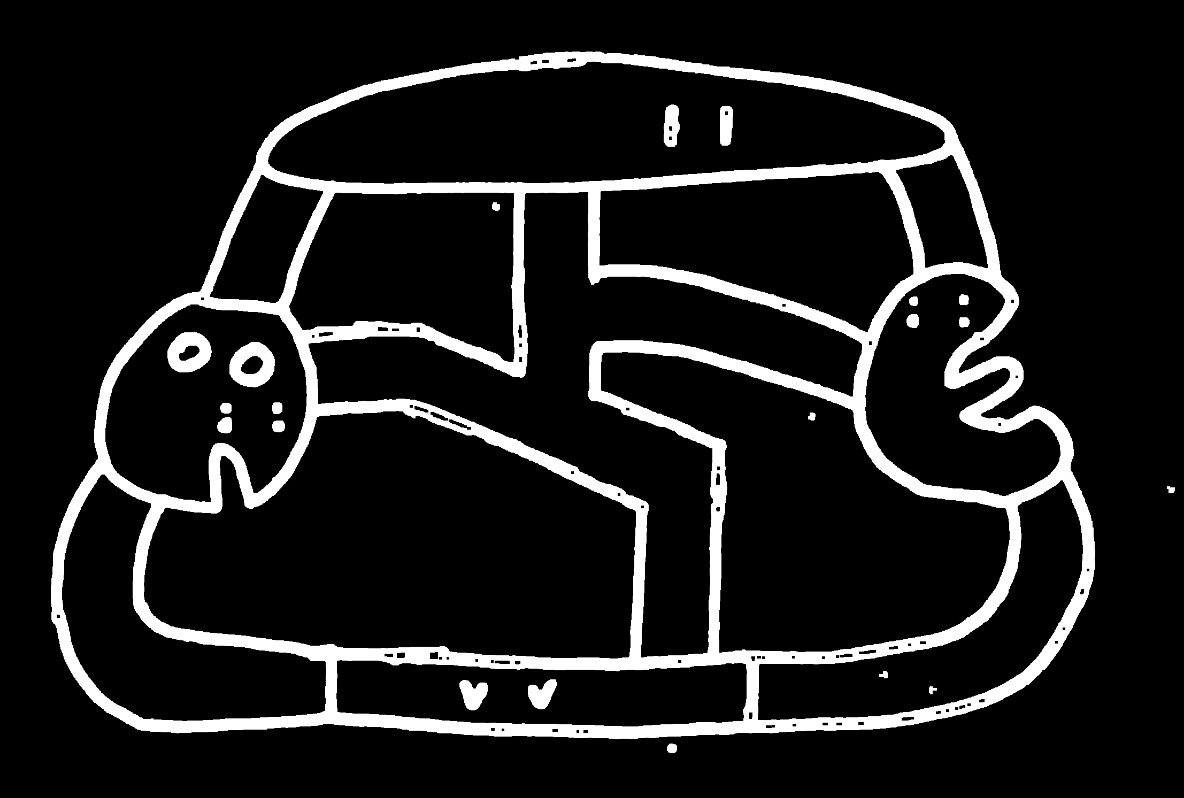
\includegraphics[width=\textwidth]{s1}
         \caption{Finding pencil}
         \label{fig:s1}
     \end{subfigure}
     \hfill
     \begin{subfigure}[b]{0.24\textwidth}
         \centering
         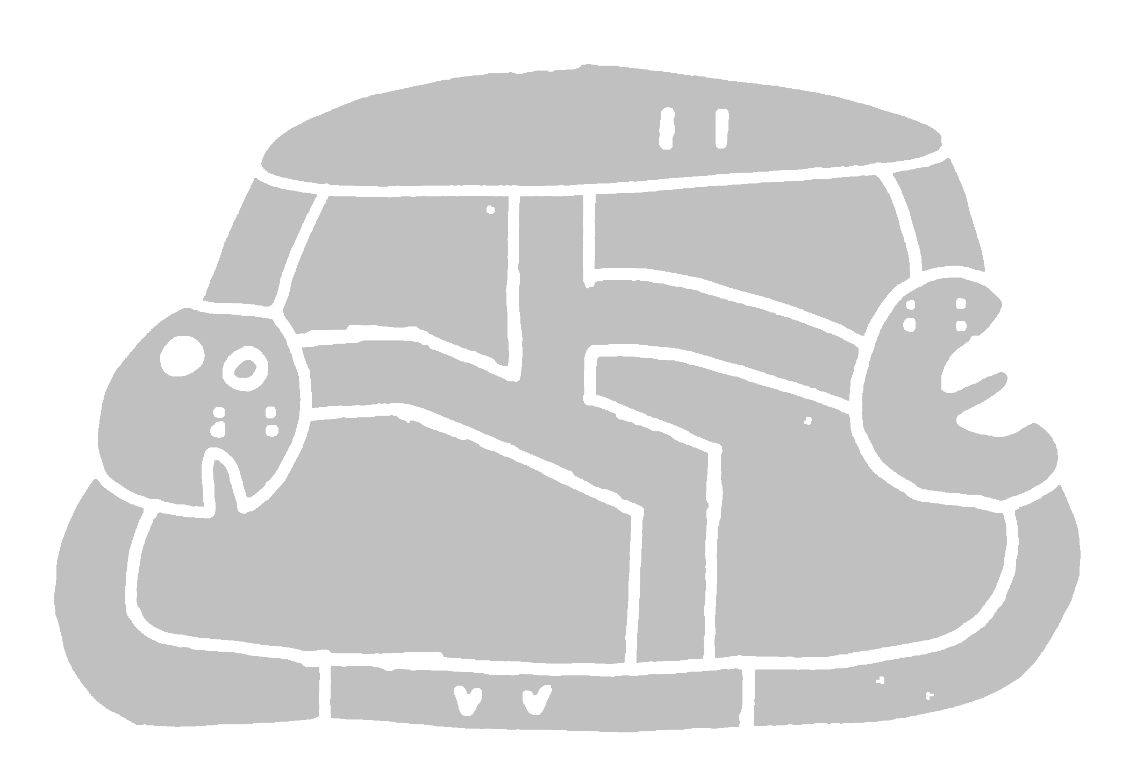
\includegraphics[width=\textwidth]{s2}
         \caption{Finding segments}
         \label{fig:s2}
     \end{subfigure}
        \caption{Segmentation}
        \label{fig:seg}
\end{figure}

\subsection{Text Recognition}
Short handwritten text is used to label segments based on what they will be in the map (floors, walls etc.). We aim to locate text precisely enough for labelling, and recognise the handwritten letters. 

The common method of detecting text with EAST and recognising text with Tesseract was tried. It was found to work best with longer words. On single letters and 2 letter words it was unreliable. Our application requires short labels (up to 2 letters at most), so this approach was unsuitable.

Instead convolution methods were tried. Inverted samples of handwritten letters were turned into kernels of various scales and convolved over the inverted image, with the idea being that highlights in the output showed presence of the letter. This detected well, but structural features in the sketches were also detected as text. Convolution by its definition rewards white overlap but does not reward black overlap, and does not explicitly punish opposites. For example a solid rectangle of pencil would be detected as any sampled letter. A more specific sort of convolution is needed.

\begin{figure}[h]
     \centering
     \begin{subfigure}[b]{0.15\textwidth}
         \centering
         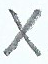
\includegraphics[width=\textwidth]{tem1}
         \caption{A single sample of the letter X}
         \label{fig:tem1}
     \end{subfigure}
     \hfill
     \begin{subfigure}[b]{0.15\textwidth}
         \centering
         
\includegraphics[width=\textwidth]{tem2}
         \caption{Multiple samples averaged}
         \label{fig:tem2}
     \end{subfigure}
     \begin{subfigure}[b]{0.15\textwidth}
         \centering
         
\includegraphics[width=\textwidth]{tem3}
         \caption{Template used in template matching}
         \label{fig:tem3}
     \end{subfigure}
     \hfill
        \caption{Template for the letter X}
        \label{fig:tem}
\end{figure}

Template matching gives us the specificity needed by rewarding pixel similarity and punishing dissimilarity. Squared difference template matching was used with the sampled letters at various scales over the image, to produce a mostly whitish image with black spots where letters are found. An example template is shown in Figure \ref{fig:tem}. This is inverted and thresholded so that only confident highlights are retained. These highlights from all scales are merged into one image (as a weighted average where every scale has the same weight). It was found that each true highlight tends to appear on multiple scales, so thresholding this merged image retains these and discards some random highlights. Suzuki et al. \cite{suzuki1985topological} contour finding algorithm is used to find the location of remaining highlights. As a further step of narrowing down true highlights, on the sketch we use double letters as labels (e.g. "XX"). So we look for pairs of highlights within a certain distance and angle range. The midpoint of each pair and the letter is recorded. This gives us the text label letters and locations. Figure \ref{fig:text} shows this process.

\begin{figure}[h]
     \centering
     \begin{subfigure}[b]{0.24\textwidth}
         \centering
         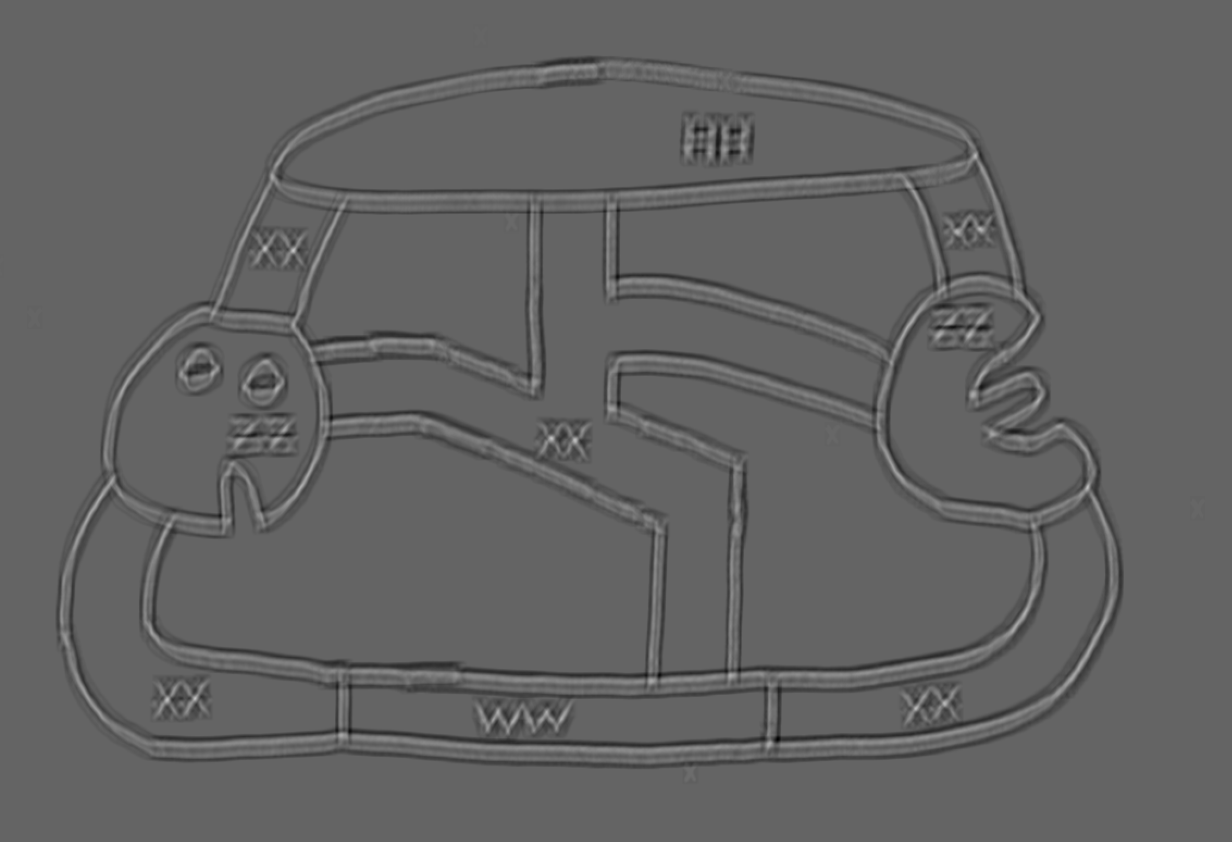
\includegraphics[width=\textwidth]{t1}
         \caption{Squared difference template match of the letter X}
         \label{fig:t1}
     \end{subfigure}
     \hfill
     \begin{subfigure}[b]{0.24\textwidth}
         \centering
         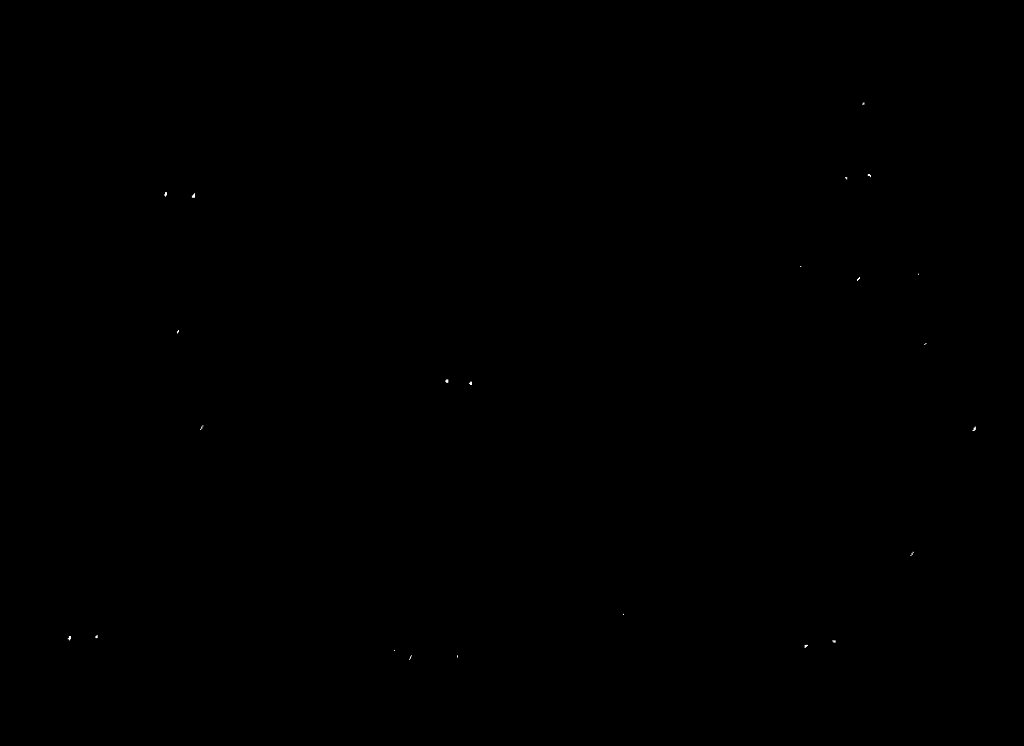
\includegraphics[width=\textwidth]{t2}
         \caption{Single scale detections (letter X)}
         \label{fig:t2}
     \end{subfigure}
     \begin{subfigure}[b]{0.24\textwidth}
         \centering
         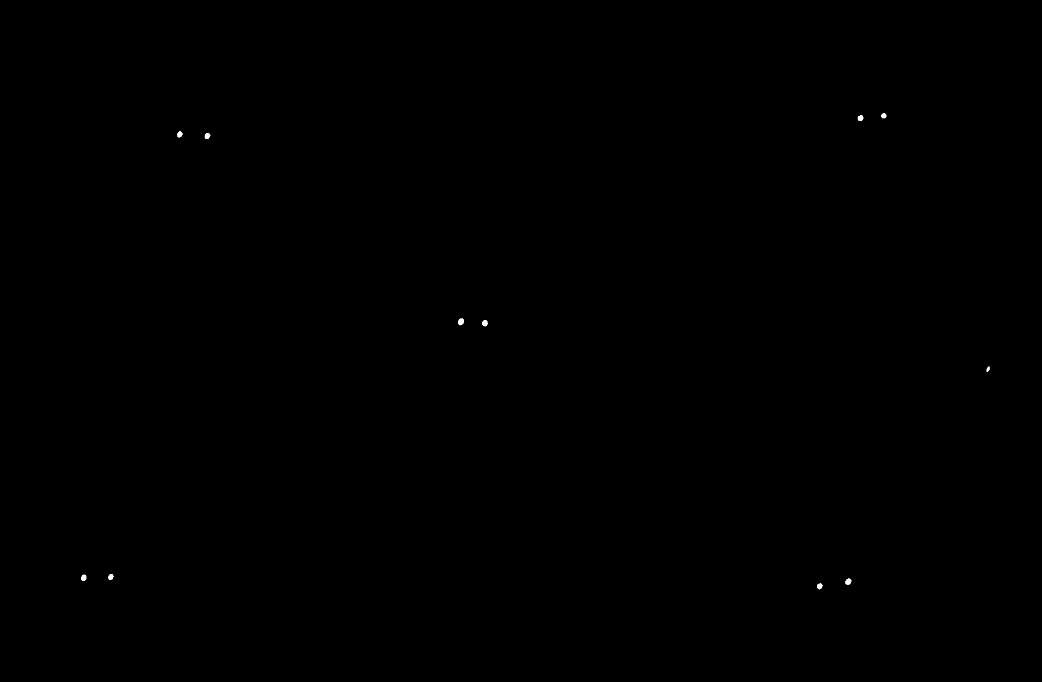
\includegraphics[width=\textwidth]{t3}
         \caption{Confidence across multiple scales (letter X)}
         \label{fig:t3}
     \end{subfigure}
     \hfill
     \begin{subfigure}[b]{0.24\textwidth}
         \centering
         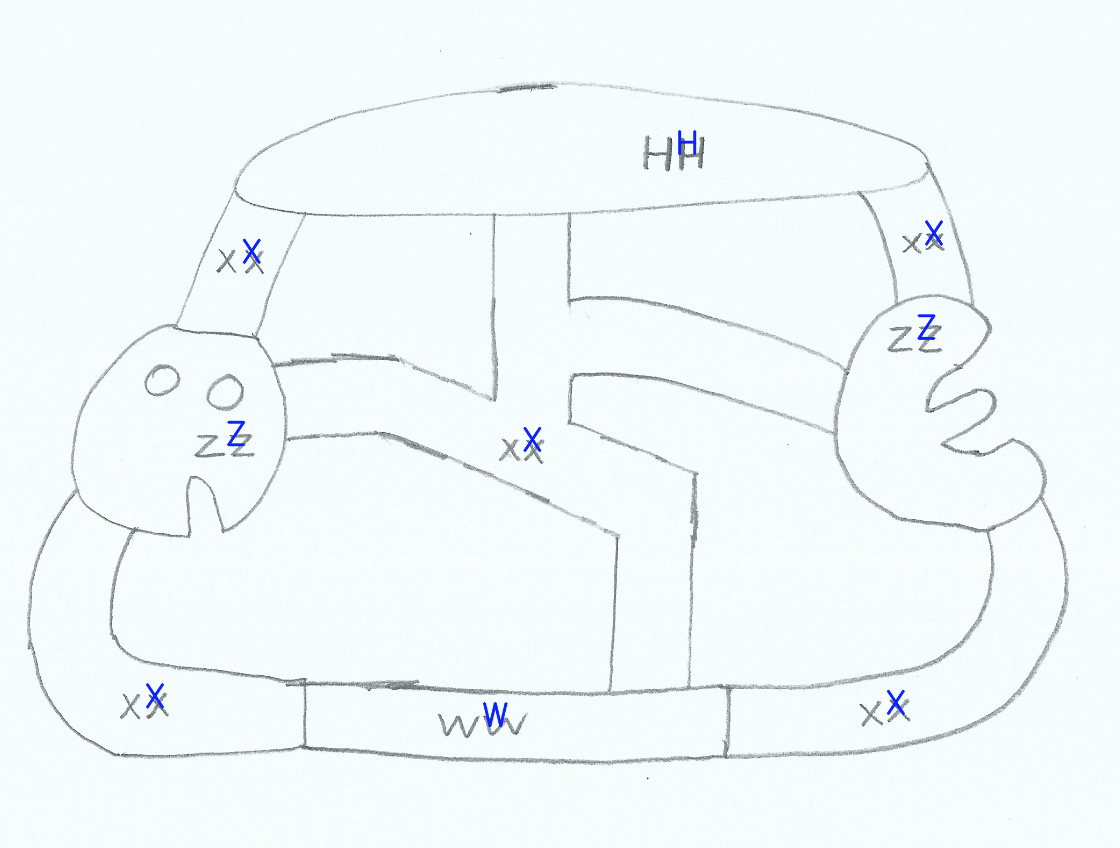
\includegraphics[width=\textwidth]{t4}
         \caption{Detected Pairs}
         \label{fig:t4}
     \end{subfigure}
        \caption{Text detection and recognition through template matching}
        \label{fig:text}
\end{figure}

\subsection{Labelling and Gap Filling}

From the segments and text labels we want to produce an image where each label has a certain colour, and each segment with that label is coloured that way. See Figure \ref{fig:labelling}.

Prior to segmentation, for each text label we fill a white rectangle over it so it isn't interpreted as a structural segment. This does not need to perfectly cover the text, but does need to reach the top and bottom of the text, so that flood filling and pencil gap filling work later.

After segmentation we colourise segments. For each text label, we use a user-defined lookup table to find its colour, then flood fill that colour from the label's location. This gives an image where labelled segments are coloured, background and pencil is white, and unlabelled segments are gray. From this point on we consider background and unlabelled segments to be "wall". We replace white and gray with black as they can be treated as the same from now on. To improve efficiency of the gap filling step we crop down the image to remove extraneous background, and scale the image down (the loss in precision is irrelevant when compared to the inaccuracy in segmentation). 

We want to fill in the black gaps left by pencil marks, both between segments (intended structural marks) and within segments (typically produced by uncovered text). For this we make PENCIL\_THICKNESS passes over the image, where PENCIL\_THICKNESS is half the width of the widest pencil mark we need to cover. In each pass if a black pixel has a coloured neighbour, it becomes that colour. This slowly grows the coloured segments until they meet each other, removing inter-segment gaps. It also fills in internal holes. After this step any remaining black segments are considered to be wall, and filled in with the "wall" colour. This gives a simplified image with colourised segments for the rest of the program to operate on. See Figure \ref{fig:labelling}.

\begin{figure}[h]
     \centering
     \begin{subfigure}[b]{0.24\textwidth}
         \centering
         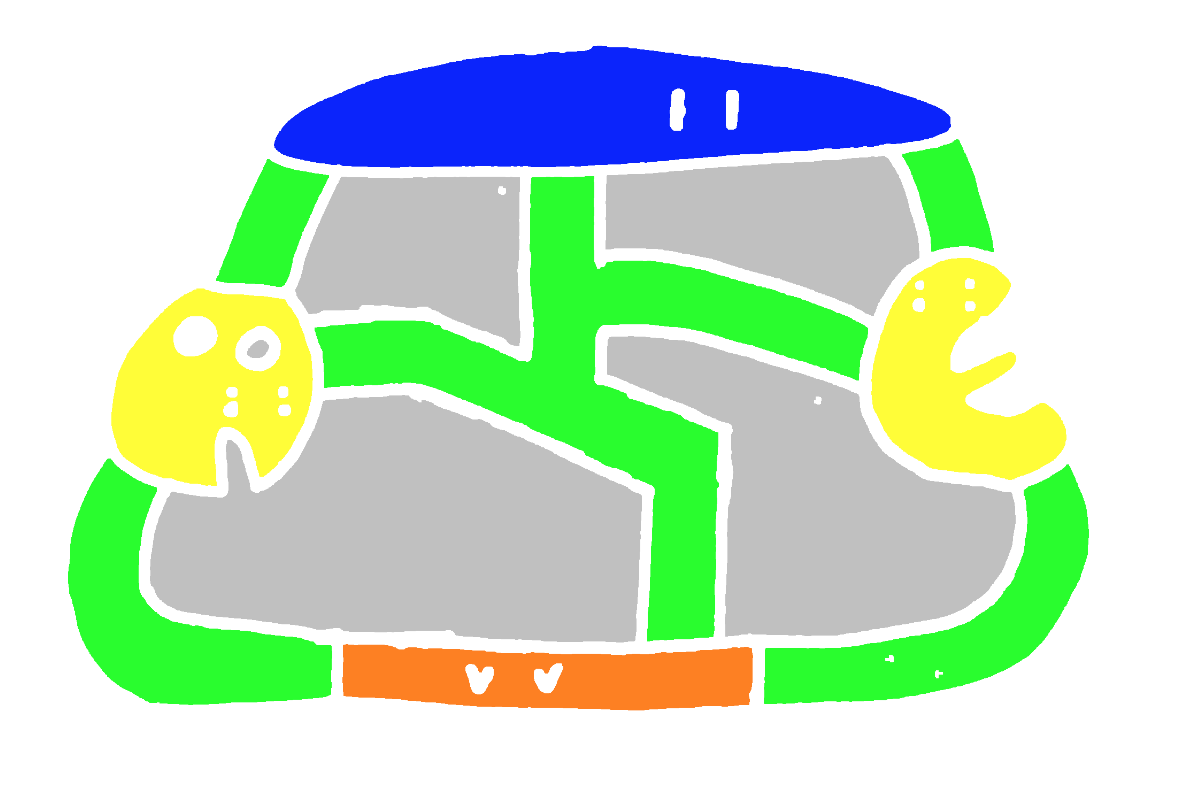
\includegraphics[width=\textwidth]{l1}
         \caption{Colouring segments using text labels}
         \label{fig:l1}
     \end{subfigure}
     \hfill
     \begin{subfigure}[b]{0.24\textwidth}
         \centering
         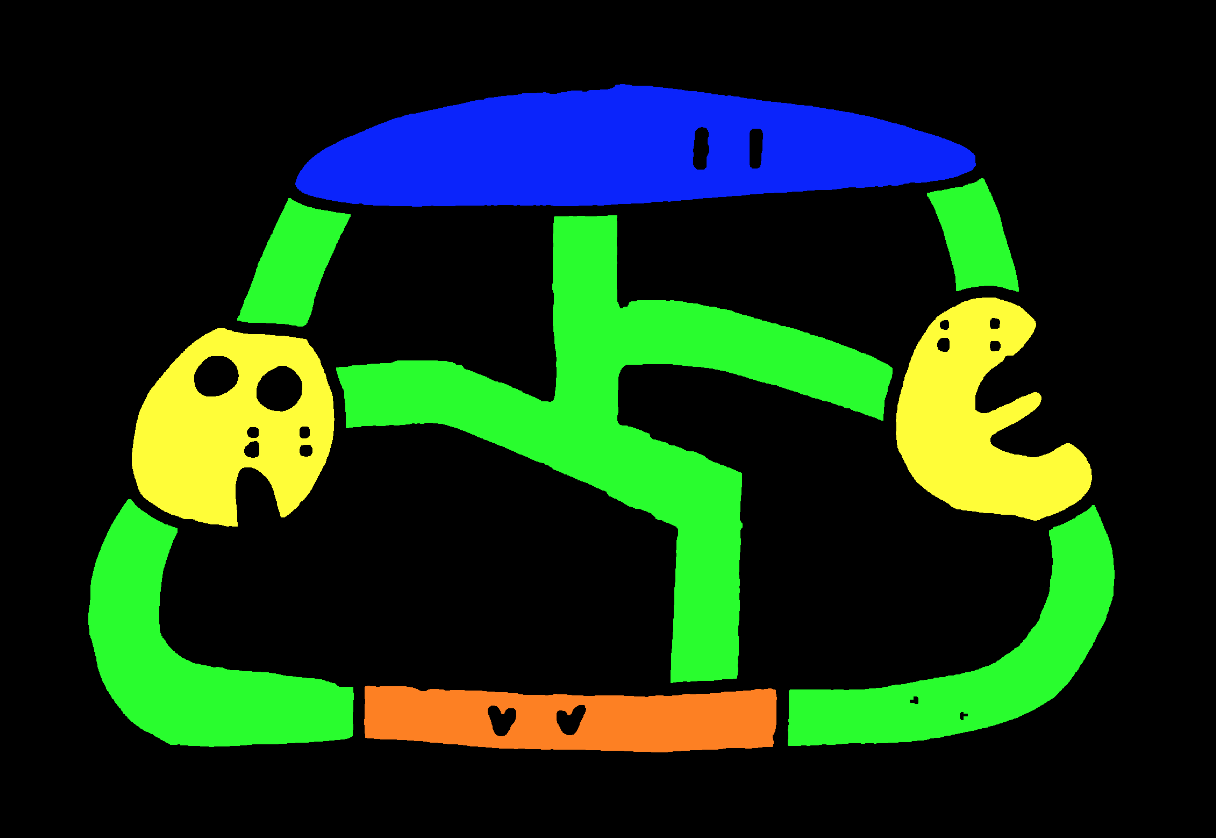
\includegraphics[width=\textwidth]{l2}
         \caption{Replacing unknown regions with black}
         \label{fig:l2}
     \end{subfigure}
     \begin{subfigure}[b]{0.24\textwidth}
         \centering
         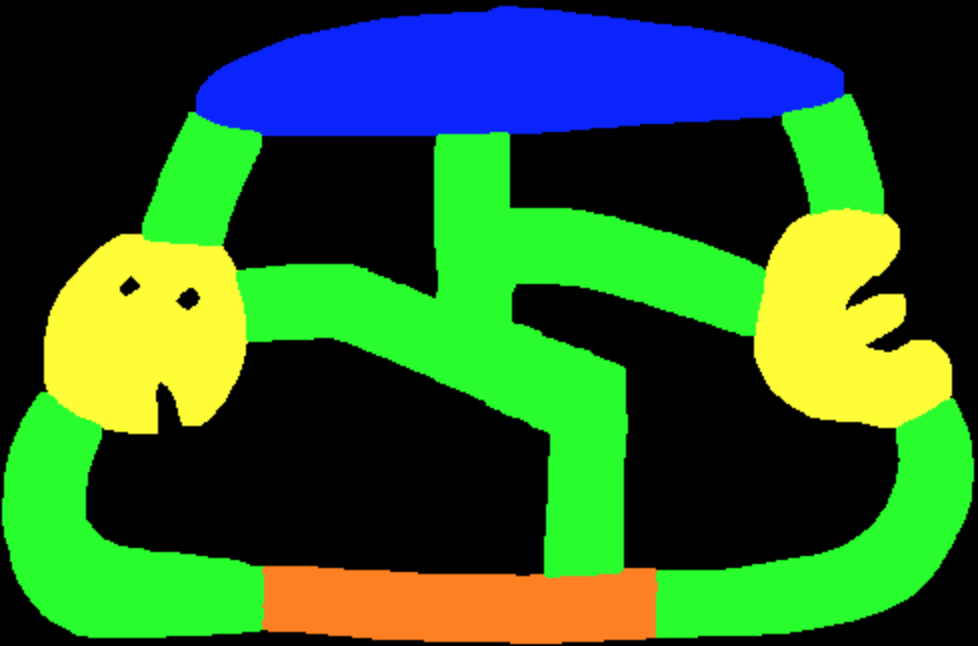
\includegraphics[width=\textwidth]{l3}
         \caption{Gap filling through dilation}
         \label{fig:l3}
     \end{subfigure}
     \hfill
     \begin{subfigure}[b]{0.24\textwidth}
         \centering
         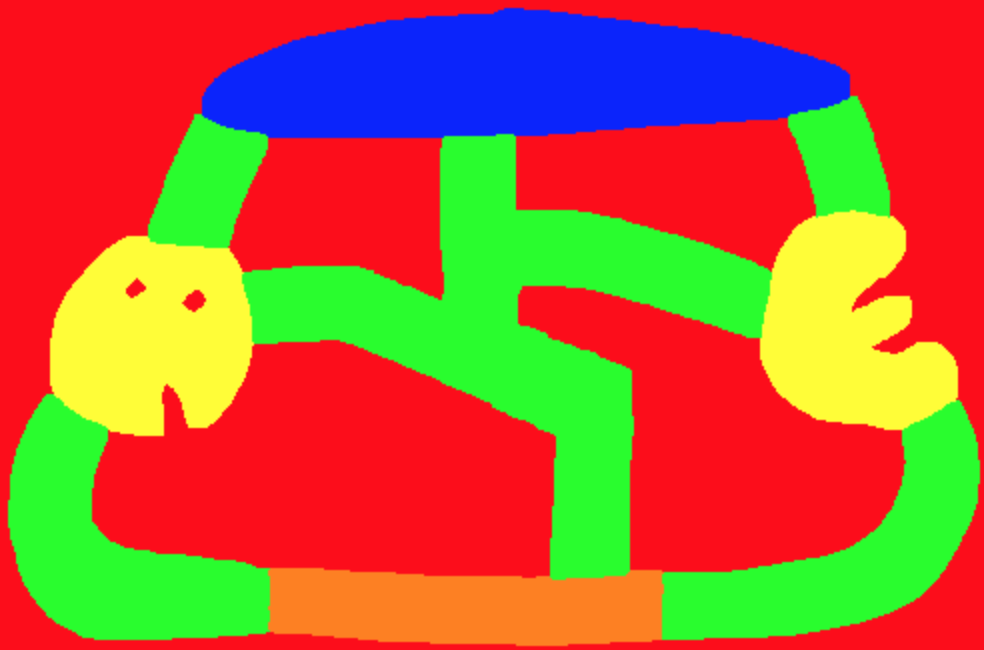
\includegraphics[width=\textwidth]{l4}
         \caption{Remaining segments coloured as wall}
         \label{fig:l4}
     \end{subfigure}
        \caption{Segment labelling and gap filling}
        \label{fig:labelling}
\end{figure}

\subsection{Segment Bordering and Triangulation}

We aim to find the border of each coloured segment, simplify it, and triangulate it to make brushes for the map file. This section operates independently of the prior sketch processing so that computer drawn images can be used.

Flood fill is used to find the pixels in each segment. A simple border walk is used to find the exact pixel by pixel border. Borders are simplified with a tolerance as a proportion of the area of the segment. Some preprocessing passes are made which operate locally, to reduce complexity. Firstly for any 3 collinear points the middle point is removed. Secondly when a corner of 1 pixel in width or height is encountered, the corner point is removed. After this, tolerance based removals are applied globally, each time looking for the point which when removed changes the segment area the least. Only concavities are removed, which is suitable in this context as it ensures no gaps between the final map objects.

The colour of segments are used as labels to generate map objects. Map objects have borders and a type (wall, floor etc.). For each object its border is triangulated. This uses a fairly simple approach of cycling around the border looking for valid triangles (counter-clockwise, not intersecting the border's edges, and not containing another border point). A valid triangle is added to the result. The polygons left over from removing this triangle are themselves triangulated recursively to find the remaining triangles. 


\section{Results}

\subsection{Setup}
OS: macOS 10.13.4

Processor: 2.4 GHz dual core I5-4258U

IDE: Visual Studio Code

Language: Python 3.7.2

Device: PC

Camera: 300dpi printer scanner (Deskjet 3070 B611)

OpenCV Version: 4.5.1

\subsection{Segmentation}

Segmentation accuracy was tested with Hamming distance, comparing against a manual segmentation. In proportion to the size of the image, there was an 8.0\% difference between the algorithmic segmentation and the manual segmentation. For reference two different manual segmentations had a 2.6\% difference. We can visually inspect Figure \ref{fig:segtest} to see that the algorithmic segmentation thins walls (red) and thickens non-walls (other colours), which accounts for the larger difference.

\begin{figure}[h]
     \centering
     \begin{subfigure}[b]{0.23\textwidth}
         \centering
         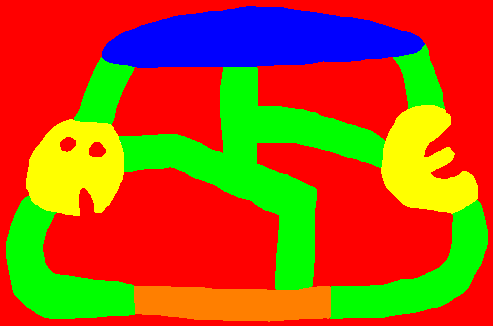
\includegraphics[width=\textwidth]{manualseg}
         \caption{Manual Segmentation}
         \label{fig:manualseg}
     \end{subfigure}
     \hfill
     \begin{subfigure}[b]{0.23\textwidth}
         \centering
         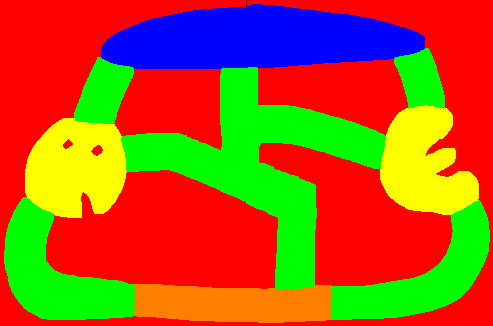
\includegraphics[width=\textwidth]{outputseg}
         \caption{Our Segmentation}
         \label{fig:outputseg}
     \end{subfigure}
        \caption{Segmentation comparison}
        \label{fig:segtest}
\end{figure}

A better solution would treat the pencil filling stage (which acts on non-wall) as a closing operation rather than just a dilation.

Segmentation took roughly 3 minutes, and the pencil filling passes (with downscaling of 4) took 32 seconds. If the original image is $W*H$ in size, and each side is scaled down by a parameter $S$, the pencil filling has complexity $O({W*H}/{S^3})$. This is because the image size is reduced by $S^2$, and the pencil gaps decrease in size by $S$ so fewer passes are required. Indeed the pencil filling runs much faster after scaling down by 4 (without scaling it took 38 minutes!), although I wouldn't scale down much further than this.

\subsection{Text Recognition}

The commonly described EAST + Tesseract method detects 90\% of double characters but only recognises 30\% of them due to its dependency on recognising complete words. Our method using sample template matching detects and recognises 100\% of double characters, with no false detections on other lines. With this method not all letters are usable as some letters detect each other. For a comparison of methods see Figure \ref{fig:texttest}.

\begin{figure}[h]
     \centering
     \begin{subfigure}[b]{0.4\textwidth}
         \centering
         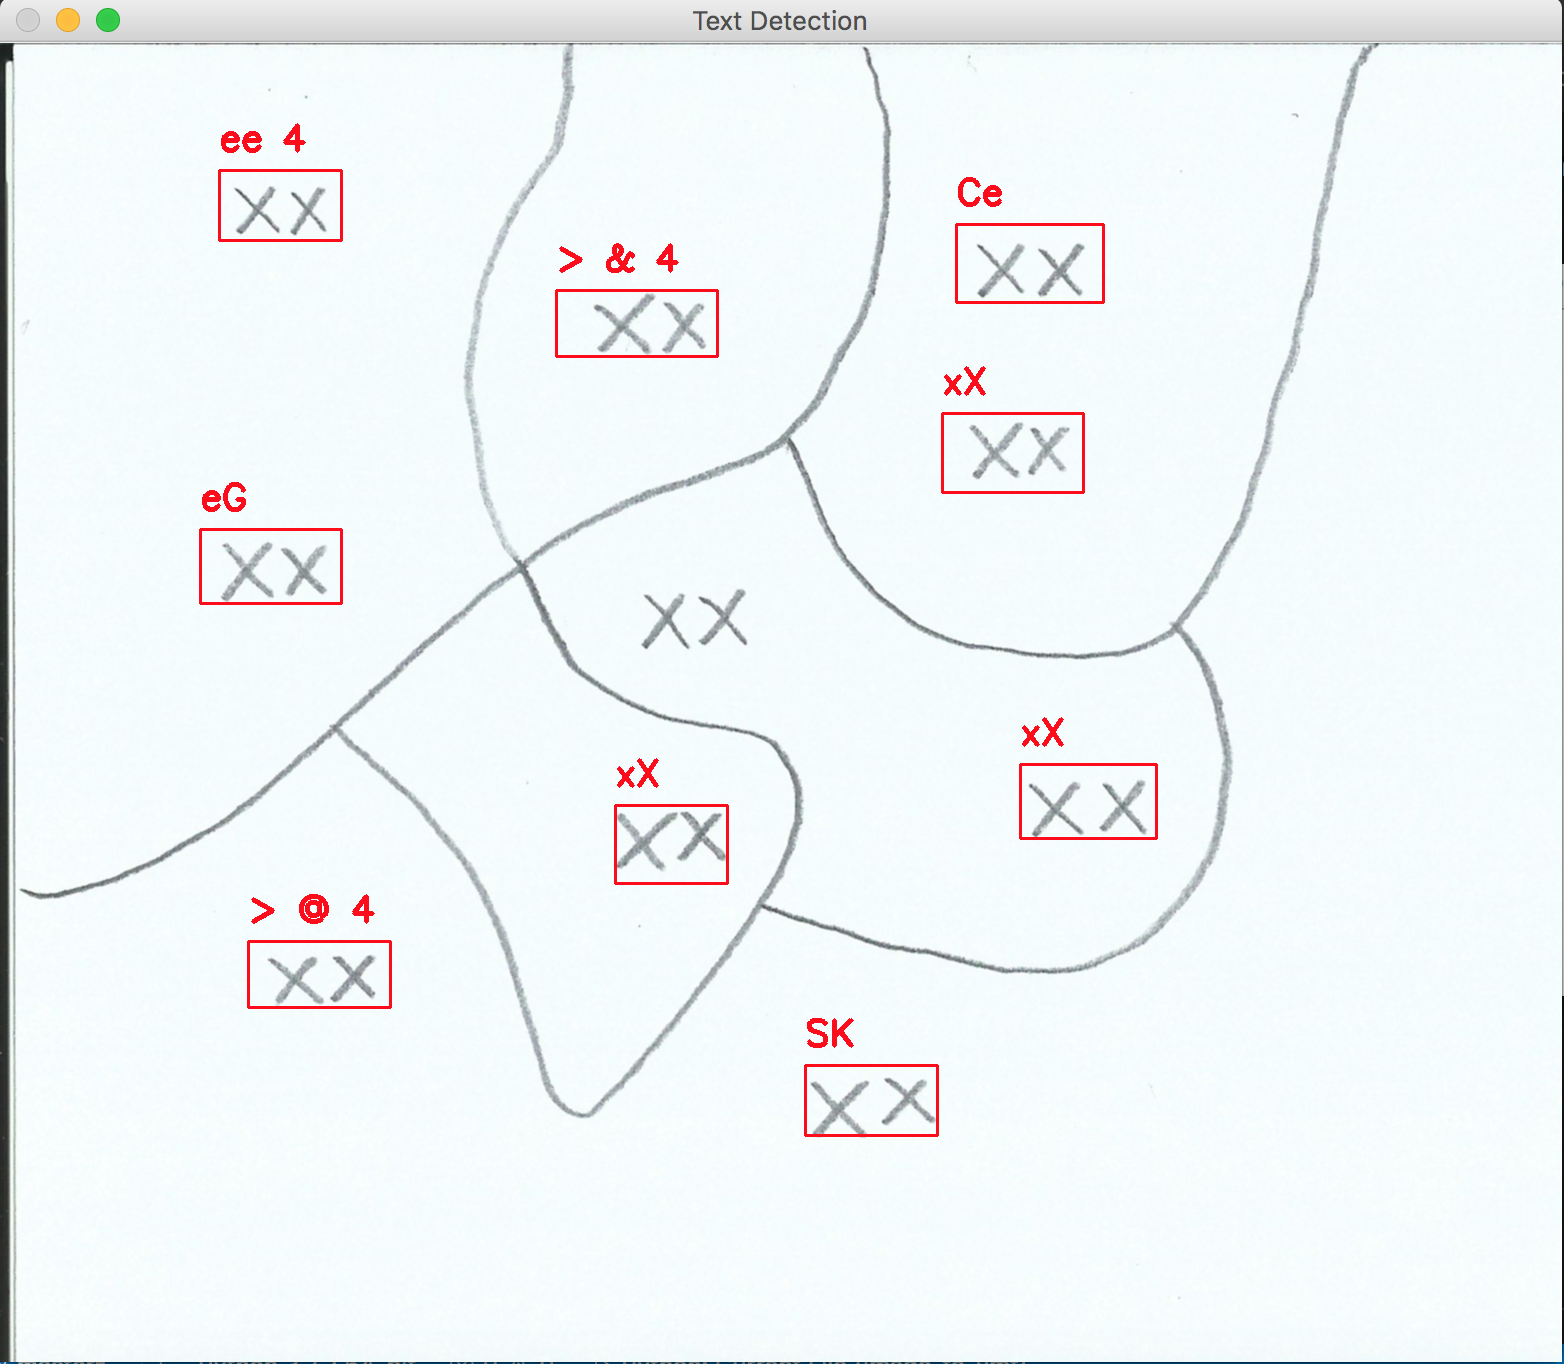
\includegraphics[width=\textwidth]{ocrprior}
         \caption{Common OCR Method}
         \label{fig:ocrprior}
     \end{subfigure}
     \hfill
     \begin{subfigure}[b]{0.4\textwidth}
         \centering
         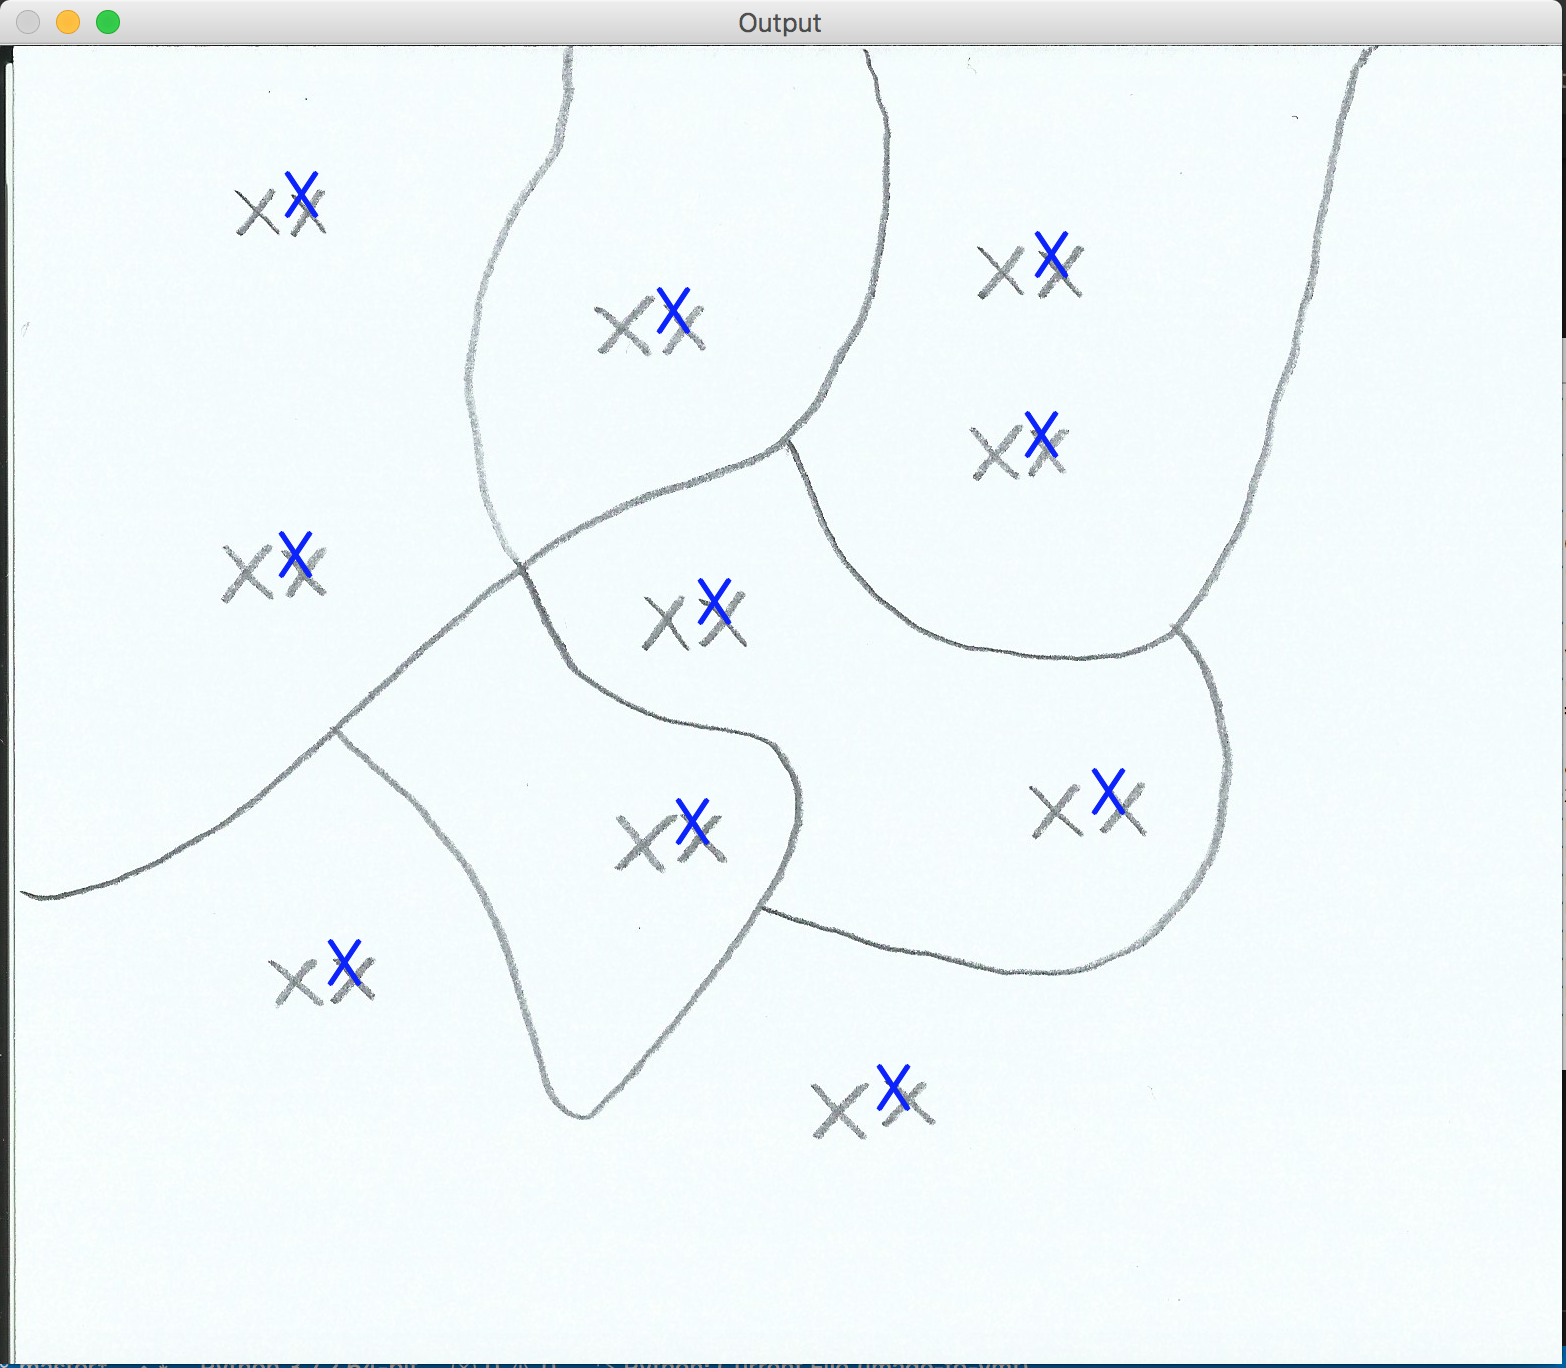
\includegraphics[width=\textwidth]{textrec}
         \caption{Our Sample Recognition}
         \label{fig:textrec}
     \end{subfigure}
        \caption{Text detection and recognition}
        \label{fig:texttest}
\end{figure}

On the sample image in Figure \ref{fig:texttest} the EAST + Tesseract method takes just 5 seconds to complete, whereas our method takes 43 seconds. For an image $W*H$, template symbols $M*N$, and number of template rescalings $X*Y$, our method has complexity $O(W*H*M*N*X*Y)$. On A4 pages at 300 ppi, our method takes about 3-4 minutes for text recognition. Template size isn't feasible to adjust, however image size and template rescalings are. Image size can be adjusted by manual cropping after scanning. Simply downscaling the image and templates makes detection more sensitive, so parameters need to be adjusted alongside this. Number of template rescalings can be reduced by consistently drawing letters at similar sizes, and setting tighter bounds on their possible size.

\subsection{Border Simplification and Triangulation}

As seen in Figure \ref{fig:tri}, our triangulation method gives triangle fans for convex polygons, and suitably handles more complicated polygons. The number of vertices is low enough as a result of the border simplification, well within what the engine can handle.

\begin{figure}[h]
     \centering
     \begin{subfigure}[b]{0.45\textwidth}
         \centering
         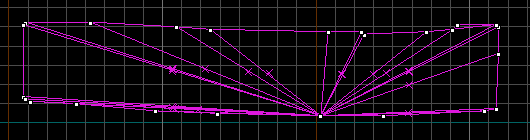
\includegraphics[width=\textwidth]{tri1}
         \caption{An almost convex polygon}
         \label{fig:tri1}
     \end{subfigure}
     \hfill
     \begin{subfigure}[b]{0.45\textwidth}
         \centering
         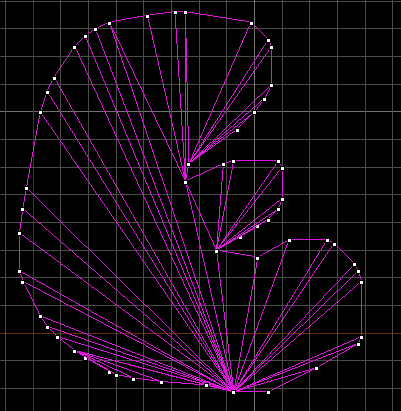
\includegraphics[width=\textwidth]{tri2}
         \caption{A polygon with concavities}
         \label{fig:tri2}
     \end{subfigure}
        \caption{Triangulation of segments}
        \label{fig:tri}
\end{figure}

With the $493*326$ simplified segmentation, the rest of the program (border marching, simplification, triangulation, and VMF construction) takes just 10 seconds. The scaling down done by pencil filling benefits this, as smaller segments with smaller borders are processed much faster. The global border simplification and triangulation can be $O(N^2)$ (better solutions are $O(N*log(N))$, so simple optimisations like these and local border simplification do a lot to help with efficiency. For example without scaling down at pencil filling, this part of the program takes 77 seconds to complete. Without local border simplification, this part takes on the order of hours. Fortunately these local border optimisations make good assumptions about the nature of the input border (several straight lines and jagged diagonal pixel lines) to remove unnecessary points immediately.

\section{Conclusion}

Pencil sketches of map layouts were segmented and coloured based on text labels. Segmentation was achieved through a robust pencil finding method, and flood filling between pencil. Text recognition was achieved through template matching of hand drawn letter samples. 

The segmentation came within 8.0\% of a reference segmentation, with no topology differences. The text recognition had a 100\% detection and recognition rate, with no false detections. The map produced was compilable and playable, with no errors related to brush size or shape. The total time taken to generate the map was about 7 minutes, which needs to be improved to allow users to quickly iterate on their designs.

\section{Further Research}

The approach described is a solid start to automating map creation, however there are many possible improvements. In general a C++ implementation for some of the intensive algorithms used would give a great speedup.

\subsection{Text Recognition}

At many points throughout template matching, seemingly arbitrary parameters have been chosen as they were found to correctly distinguish between letters and other structures. The margins for these parameters to work were small, and I suspect they are tuned to my exact scanning setup. To make text recognition more robust, these parameters could be investigated or made adaptive. Here are some ideas:

\begin{itemize}
\item Squared difference produces a large range of values. Currently the largest value in the output is found, and the output normalised from this value. There should be a way to calculate a theoretical "sample on plain background" or "sample on exact opposite" expected value, based on template size and colour dimensions, to consistently normalise by the same amount across all scales. 
\item We expect 1 of each team spawn and 1-3 bombsites. We could adaptively alter detection sensitivity until the correct number are detected, which will also improve detection accuracy of floors. 
\item Each letter is different in its density and similarity to other drawn structures, so each letter could be tuned with its own parameters.
\item Run a template match on the template itself to see what we'd expect to find from an exact match, and try to find similar outputs on the template matched sketch.
\end{itemize}

Performance is a key issue with template matching. GPU implementations with kernels we define based on templates, such as with CuPy \cite{cupy2015user}, could be investigated. More advanced methods such as feature descriptors could be used. Neural networks could be trained on handwritten 2 letter words for this particular application.

\subsection{Segmentation}

There is a small margin between the intensity of background paper and intensity of pencil. Adaptive thresholding is used currently, but we may want to know the background and pencil intensities for other uses (the white rectangle that covers up text for example). An intensity histogram could be used, looking for two peaks representing the background and pencil intensities.

As previously mentioned, the pencil gap filling stage only acts as a dilation, resulting in enlarged non-walls and shrunken walls. If precise scales are needed, an erosion pass of the same size could be made after gaps are closed to fix the scales. Also the pencil filling stage has a fairly naive implementation, with one pass at a time looking in a $3*3$ region around each pixel. Typical morphology implementations could be extended to this colour and black situation, to improve performance. A kernel convolution solution may exist.

The white rectangle used to cover up text can be made more precise if needed in future. We could record the detection size which produced the matched pair to get the exact height needed. A marching algorithm could be used to work outwards from the centre until the outside of the text is found.

\subsection{Border Simplication and Triangulation}

Currently we border march every pixel to find an exact border, then simplify it separately. Approaches exist to border march multiple pixels at a time, effectively combining these two steps into one. Pu et al. \cite{pu2008adaptive} propose adaptive border marching to dynamically choose step sizes whilst marching around a border. Step sizes are made smaller if a larger step excludes a sufficiently large concavity or protrusion. This method retains necessary details whilst reducing vertex count. Alternatively we could keep the current 2 step algorithm and implement Douglas-Peucker \cite{douglas1973algorithms} for simplication.

Segments are currently allowed to become larger during border simplification, which overlaps brushes from different objects in the map. This is good for gameplay as there are no gaps, but it may cause unforeseen problems with the visibility algorithm or other parts of map compilation. The border simplification could be adjusted into a global algorithm, where adjacent borders share the same vertices, and removing or moving vertices applies to any segments using them in their border. So borders end up perfectly joined between segments, and brushes align perfectly in the map.

Donut topology (holes in the middle of segments) are not accounted for in the current program. As a simple fix the outer wall has a pixel of black drawn through it to break up the donut, but internal segments are still vulnerable to the issue if a user draws an object with donut topology. An accurate fix would be to find holes in segments and record them as internal borders, simplify these borders the same as the external border, then use a triangulation algorithm which can cope with internal borders. For example Shewchuk's Triangle \cite{shewchuk2005two}. A simpler fix would be to detect holes in segments, then split the segment in two, and recursively fix holes in the two new segments produced, until there are no holes remaining.

\subsection{Other Features}

Config options such as scaling and skybox texture can be added. Some way of sketching crates should be added.

CS:GO maps typically have some height variation, and even overlapping floors. A way of defining a height map through drawn elevation numbers could be added, and some way of sketching overlapping floors. Perhaps a symbol indicating where two nearby floors should be joined together could be added.

\bibliographystyle{IEEEtran}
\bibliography{references}

\end{document}